%%
%% Copyright (c) 2018-2019 Weitian LI <liweitianux@sjtu.edu.cn>
%% Creative Commons BY 4.0
%%

\chapter{射电晕辐射对 EoR 信号探测的影响}
\label{chap:halo}

利用\autoref{chap:simulation}模拟得到的射电晕、
EoR 信号以及其他前景成分的 SKA1-Low 观测图像,
可以分别针对\ac{fg-rm}和\ac{fg-avd}两类前景处理方法 (\autoref{sec:fg-methods})
评估射电晕辐射对 EoR 信号探测的影响。
首先,我们计算一维\ac{ps} $\ac{psD}(k)$ 来对比射电晕辐射和
EoR 信号在各个尺度 $k$ 的功率,
说明使用\ac{fg-rm}方法时将面临的射电晕辐射的干扰程度。
其次,我们计算二维\ac{ps} $\ac{psD}(\ac{k-perp}, \ac{k-los})$,
然后在 EoR 窗口 (\autoref{sec:eor-window}) 内比较射电晕辐射和 EoR 信号的功率,
据此评估使用\ac{fg-avd}方法提取 EoR 信号时射电晕辐射将产生的污染强度。


%=====================================================================
\section{频率维度的加窗处理}
\label{sec:window}

\begin{figure}[htp]
  \centering
  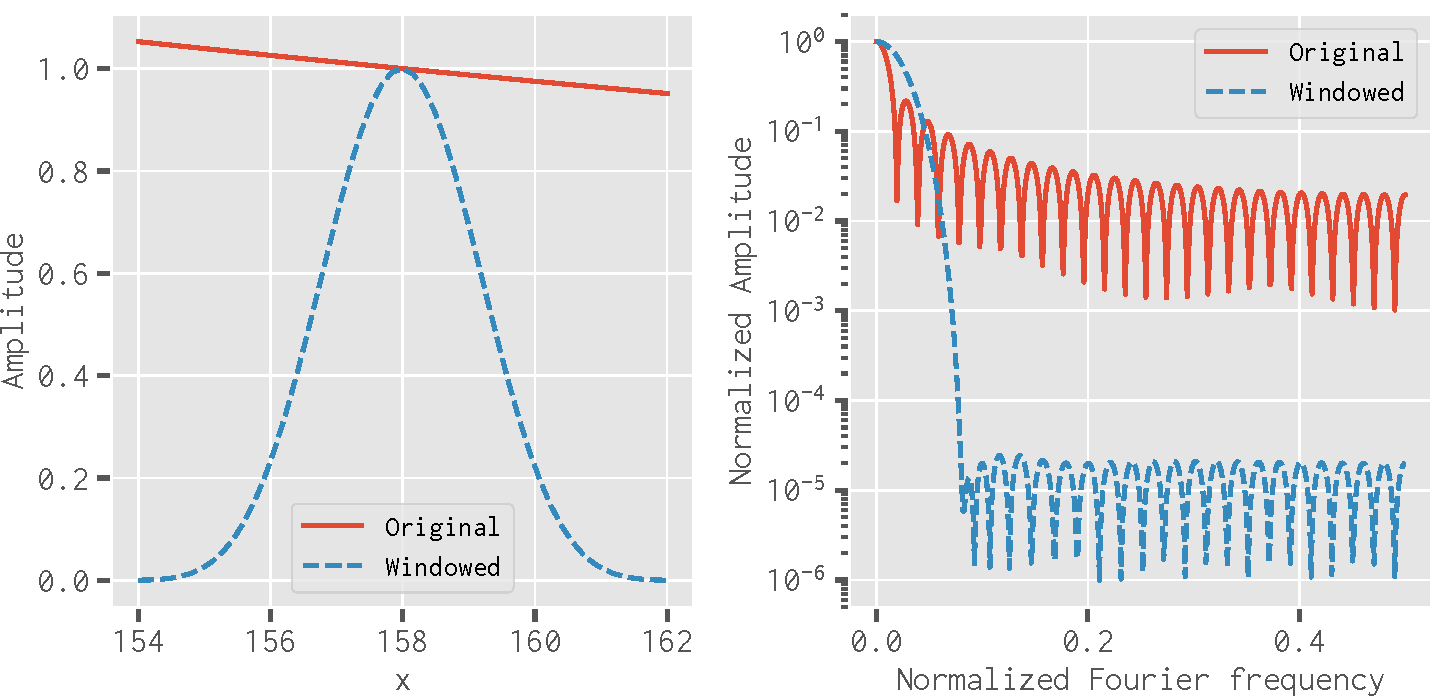
\includegraphics[width=\textwidth]{ft-sidelobes}
  \bicaption[加窗前后的 Fourier 变换结果对比]{%
    直接进行 Fourier 变换(红色实线)与
    使用 Blackman--Nuttall \acs*{f-window}之后再 Fourier 变换(蓝色虚线)
    的结果对比。
    左栏显示了原输入信号 $y = (x/158)^{-2}$ (红色实线)以及
    加窗后的输入信号(蓝色虚线),
    右栏显示了相应的 Fourier 变换结果。
  }{%
    A comparison of the Fourier transform results with and without
    applying the Blackman--Nuttall window function.
    The left panel shows the original input signal $y = (x/158)^{-2}$
    (solid red line) and the windowed signal (dashed blue line);
    the right panel shows the corresponding Fourier transform results.
  }
  \label{fig:ft-sidelobes}
\end{figure}

考虑一个有限宽的频带,信号(如前景辐射)将在频带的两端出现跃变,
这会导致 Fourier 变换的结果出现显著的\ac{sidelobe}。
即使输入信号非常平滑,Fourier 变换后也会出现一系列幅度较大的高频 Fourier 成分
(亦称为\ac{sidelobe}),如\autoref{fig:ft-sidelobes} 所示。
为了抑制这些\ac{sidelobe},可以先对信号加窗,然后再进行 Fourier 变换。
一个常用的选择是 Blackman--Nuttall \ac{f-window},
该\ac{f-window}具有良好的\ac{sidelobe}抑制效果 \cite{nuttall1981},
其表达式为:
\begin{equation}
  \label{eq:bn-window}
  w[n] = a_0 - a_1 \cos\left(\frac{2\Cpi n}{N}\right)
    + a_2 \cos\left(\frac{4\Cpi n}{N}\right)
    - a_3 \cos\left(\frac{6\Cpi n}{N}\right) ,
\end{equation}
其中
$N$ 为采样点的数目(即窗的宽度),
其他系数分别为:
$a_0 = \num{0.3635819}$,
$a_1 = \num{0.4891775}$,
$a_2 = \num{0.1365995}$,
$a_3 = \num{0.0106411}$。
\autoref{fig:ft-sidelobes} 显示了使用 Blackman--Nuttall
\ac{f-window}之后得到的 Fourier 变换结果,
可见高频 Fourier 成分的幅度被有效地抑制了。
因此,我们对\autoref{chap:simulation}模拟得到的\ac{imgcube}沿频率方向施加
Blackman--Nuttall \ac{f-window},
然后再进行 Fourier 变换以及计算\ac{ps} \cite{trott2015,chapman2016}。


%=====================================================================
\section{一维功率谱的对比}
\label{sec:ps1d}

我们对上一章模拟得到的每一个成分在每一个频带里的\ac{imgcube}分别计算了
一维\ac{ps} $\ac{psD}(k)$。
对于射电晕,我们使用了 100 次模拟的全部结果 (\autoref{sec:halo-maps}) 
来估算其一维功率谱的中位值和 68\% 误差范围。
具体而言,对于每一个频带,射电晕的 100 次模拟会生成 100 个\ac{imgcube},
分别计算这 100 个\ac{imgcube}的一维功率谱,
然后从所得的 100 个一维功率谱计算每个尺度 $k$ 处的中位值和 68\% 误差范围。

\begin{figure}[htp]
  \centering
  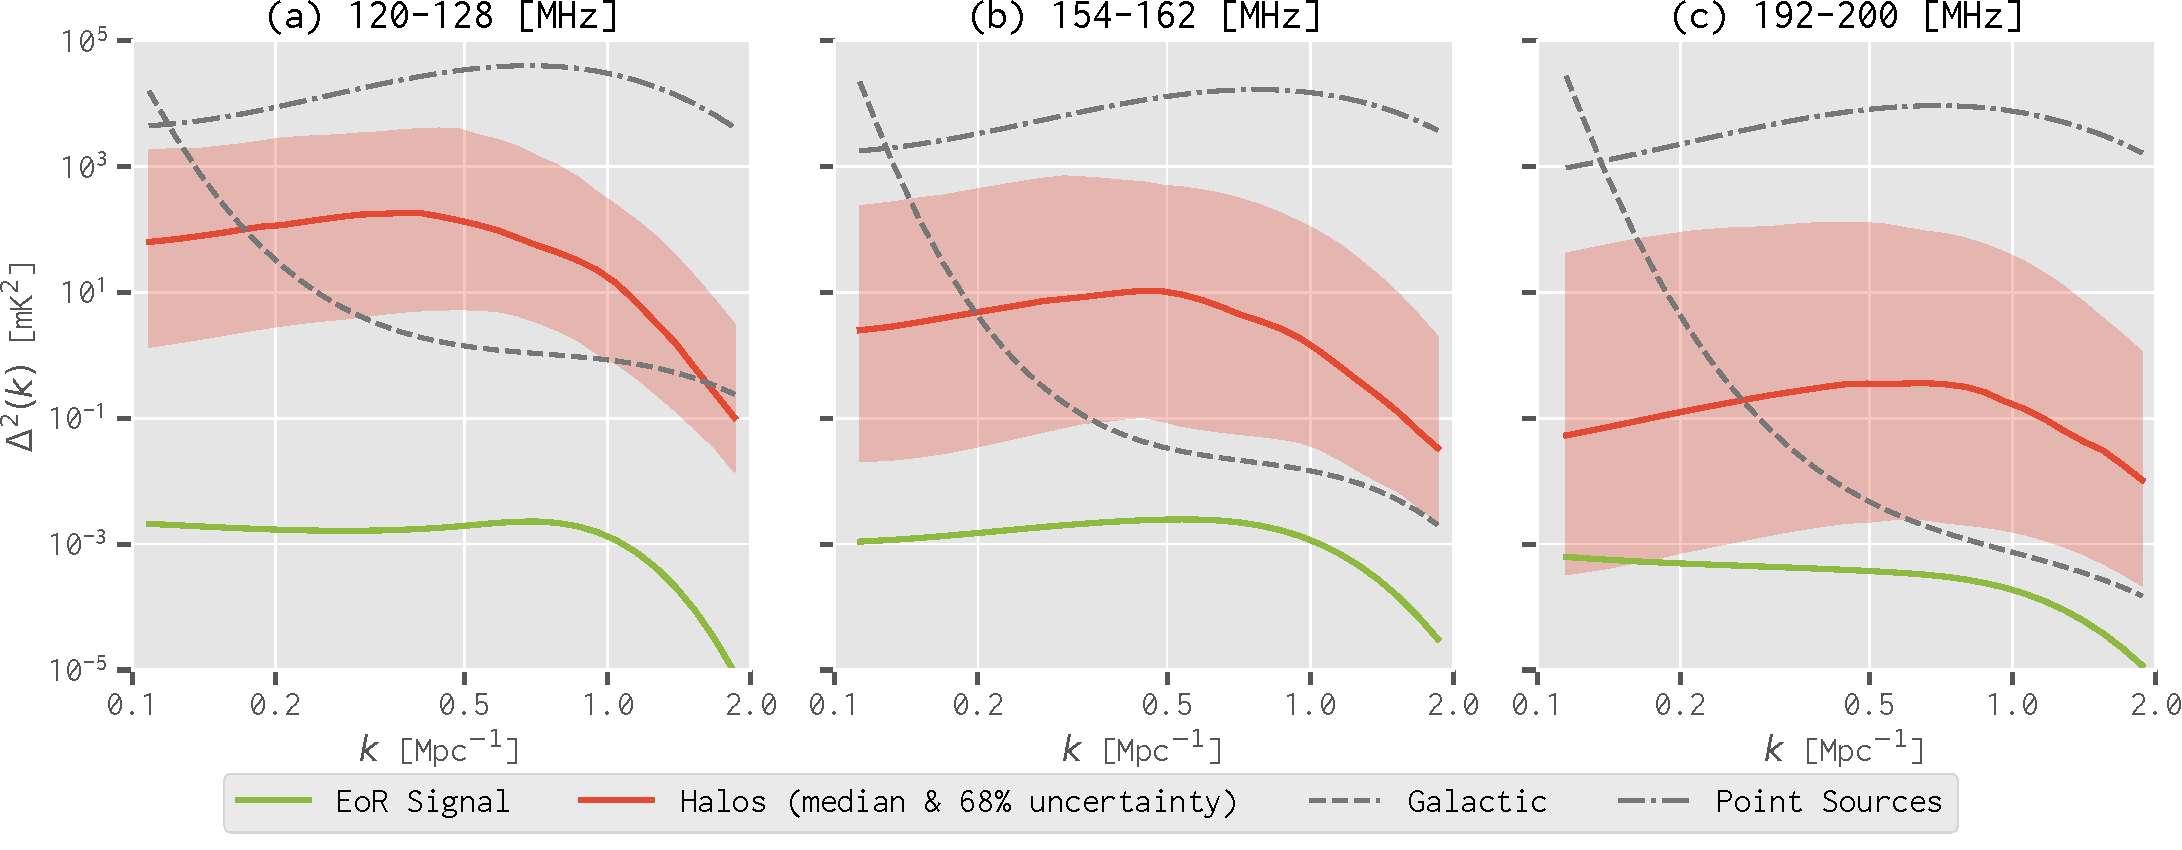
\includegraphics[width=\textwidth]{ps1d-3bands}
  \bicaption[EoR 信号和前景成分在三个频带内的一维功率谱对比]{%
    EoR 信号(绿色实线)、射电晕(红色实线)、银河系弥散辐射(灰色虚线)以及
    河外点源(灰色点虚线)之间的一维功率谱 $\ac{psD}(k)$ 的对比。
    左栏、中栏、右栏分别表示 \numrange{120}{128}、\numrange{154}{162}
    和 \numrange{192}{200} \si{\MHz} 三个频带的结果。
    对于射电晕,红色实线及其阴影区域分别表示从 100 次模拟结果得到的
    中位值和 68\% 误差范围。
  }{%
    Comparisons of the 1D dimensionless power spectra $\ac{psD}(k)$
    among the EoR signal (solid green line), radio halos (solid red line),
    Galactic diffuse emission (dashed gray line), and extragalactic point
    sources (dash-dotted gray line) in the
    \emph{(a)} \SIrange{120}{128}{\MHz},
    \emph{(b)} \SIrange{154}{162}{\MHz}, and
    \emph{(c)} \SIrange{192}{200}{\MHz} frequency bands.
    The solid red lines and shaded regions represent the median values
    and the corresponding 68\% uncertainties of the power
    spectra for radio halos estimated from the 100 simulation runs.
  }
  \label{fig:ps1d-3bands}
\end{figure}

各成分在三个频带内的一维功率谱 $\ac{psD}(k)$ 的对比
如\autoref{fig:ps1d-3bands} 所示。
我们发现,在 $\SI{0.1}{\per\Mpc} < k < \SI{2}{\per\Mpc}$ 尺度范围内,
射电晕辐射在 \numrange{120}{128}、\numrange{154}{162} 和
\numrange{192}{200} \si{\MHz} 频带内的典型功率(红色实线)
分别约为 EoR 信号功率的 \num{10000}、1000 和 300 倍。
考虑到射电晕的亮度和数目在不同天区之间会发生显著变化,
因此在 68\% 误差范围内(红色阴影区域),
射电晕辐射的功率能够变化约 \numrange{10}{100} 倍。

对于另外两个前景成分,银河系弥散辐射在最大尺度 ($k \lesssim \SI{0.1}{\per\Mpc}$)
上是最强的污染源,但随着尺度的减小(对应于 $k$ 增大),其功率迅速减小。
在 $\SI{0.5}{\per\Mpc} \lesssim k \lesssim \SI{1}{\per\Mpc}$
的中小尺度范围,
射电晕辐射的典型功率比银河系前景的功率强约 \numrange{10}{100} 倍。
河外点源除了在最大尺度上弱于银河系前景,在其他尺度上均是最强的污染源。

在射电观测研究中,更习惯使用角分或角秒来描述信号的尺度分布情况。
尺度 \ac{scale} 与\ac{wavenumber} \ac{k} 之间的换算关系与信号源的距离相关,
具体换算方法可参见附录 \autoref{sec:wavenumber-scale-conv}。
以频率为 $\nu = \SI{158}{\MHz}$ 的 EoR 信号为例,对应的中性氢云的红移为
$z = \ac{freq21cm} / \ac{freq} - 1 \approx 7.99$,
其中 \ac{freq21cm} 是\acl{freq21cm} [\autoref{eq:hi-line-frequency}],
于是可知\ac{wavenumber} $\ac{k} = \SI{1}{\per\Mpc}$
对应于尺度 $\ac{scale} = \SI{2.36}{\arcminute}$。
因此,射电晕辐射的主要功率分布尺度
$\SI{0.5}{\per\Mpc} \lesssim k \lesssim \SI{1}{\per\Mpc}$
大约对应于 \SIrange[range-units=repeat]{2.4}{4.8}{\arcminute} 的尺度,
这与射电晕的典型大小(角分至数个角分)相符。

以上这些结果清楚地说明射电晕是严重的 EoR 前景污染源,需要在前景扣除中仔细处理。
此外,射电晕的形态还呈现一定程度的不规则结构,这显著增加了对其进行准确建模和扣除的难度。


%=====================================================================
\section{二维功率谱以及 EoR 窗口的对比}
\label{sec:ps2d}

\begin{figure}[htp]
  \centering
  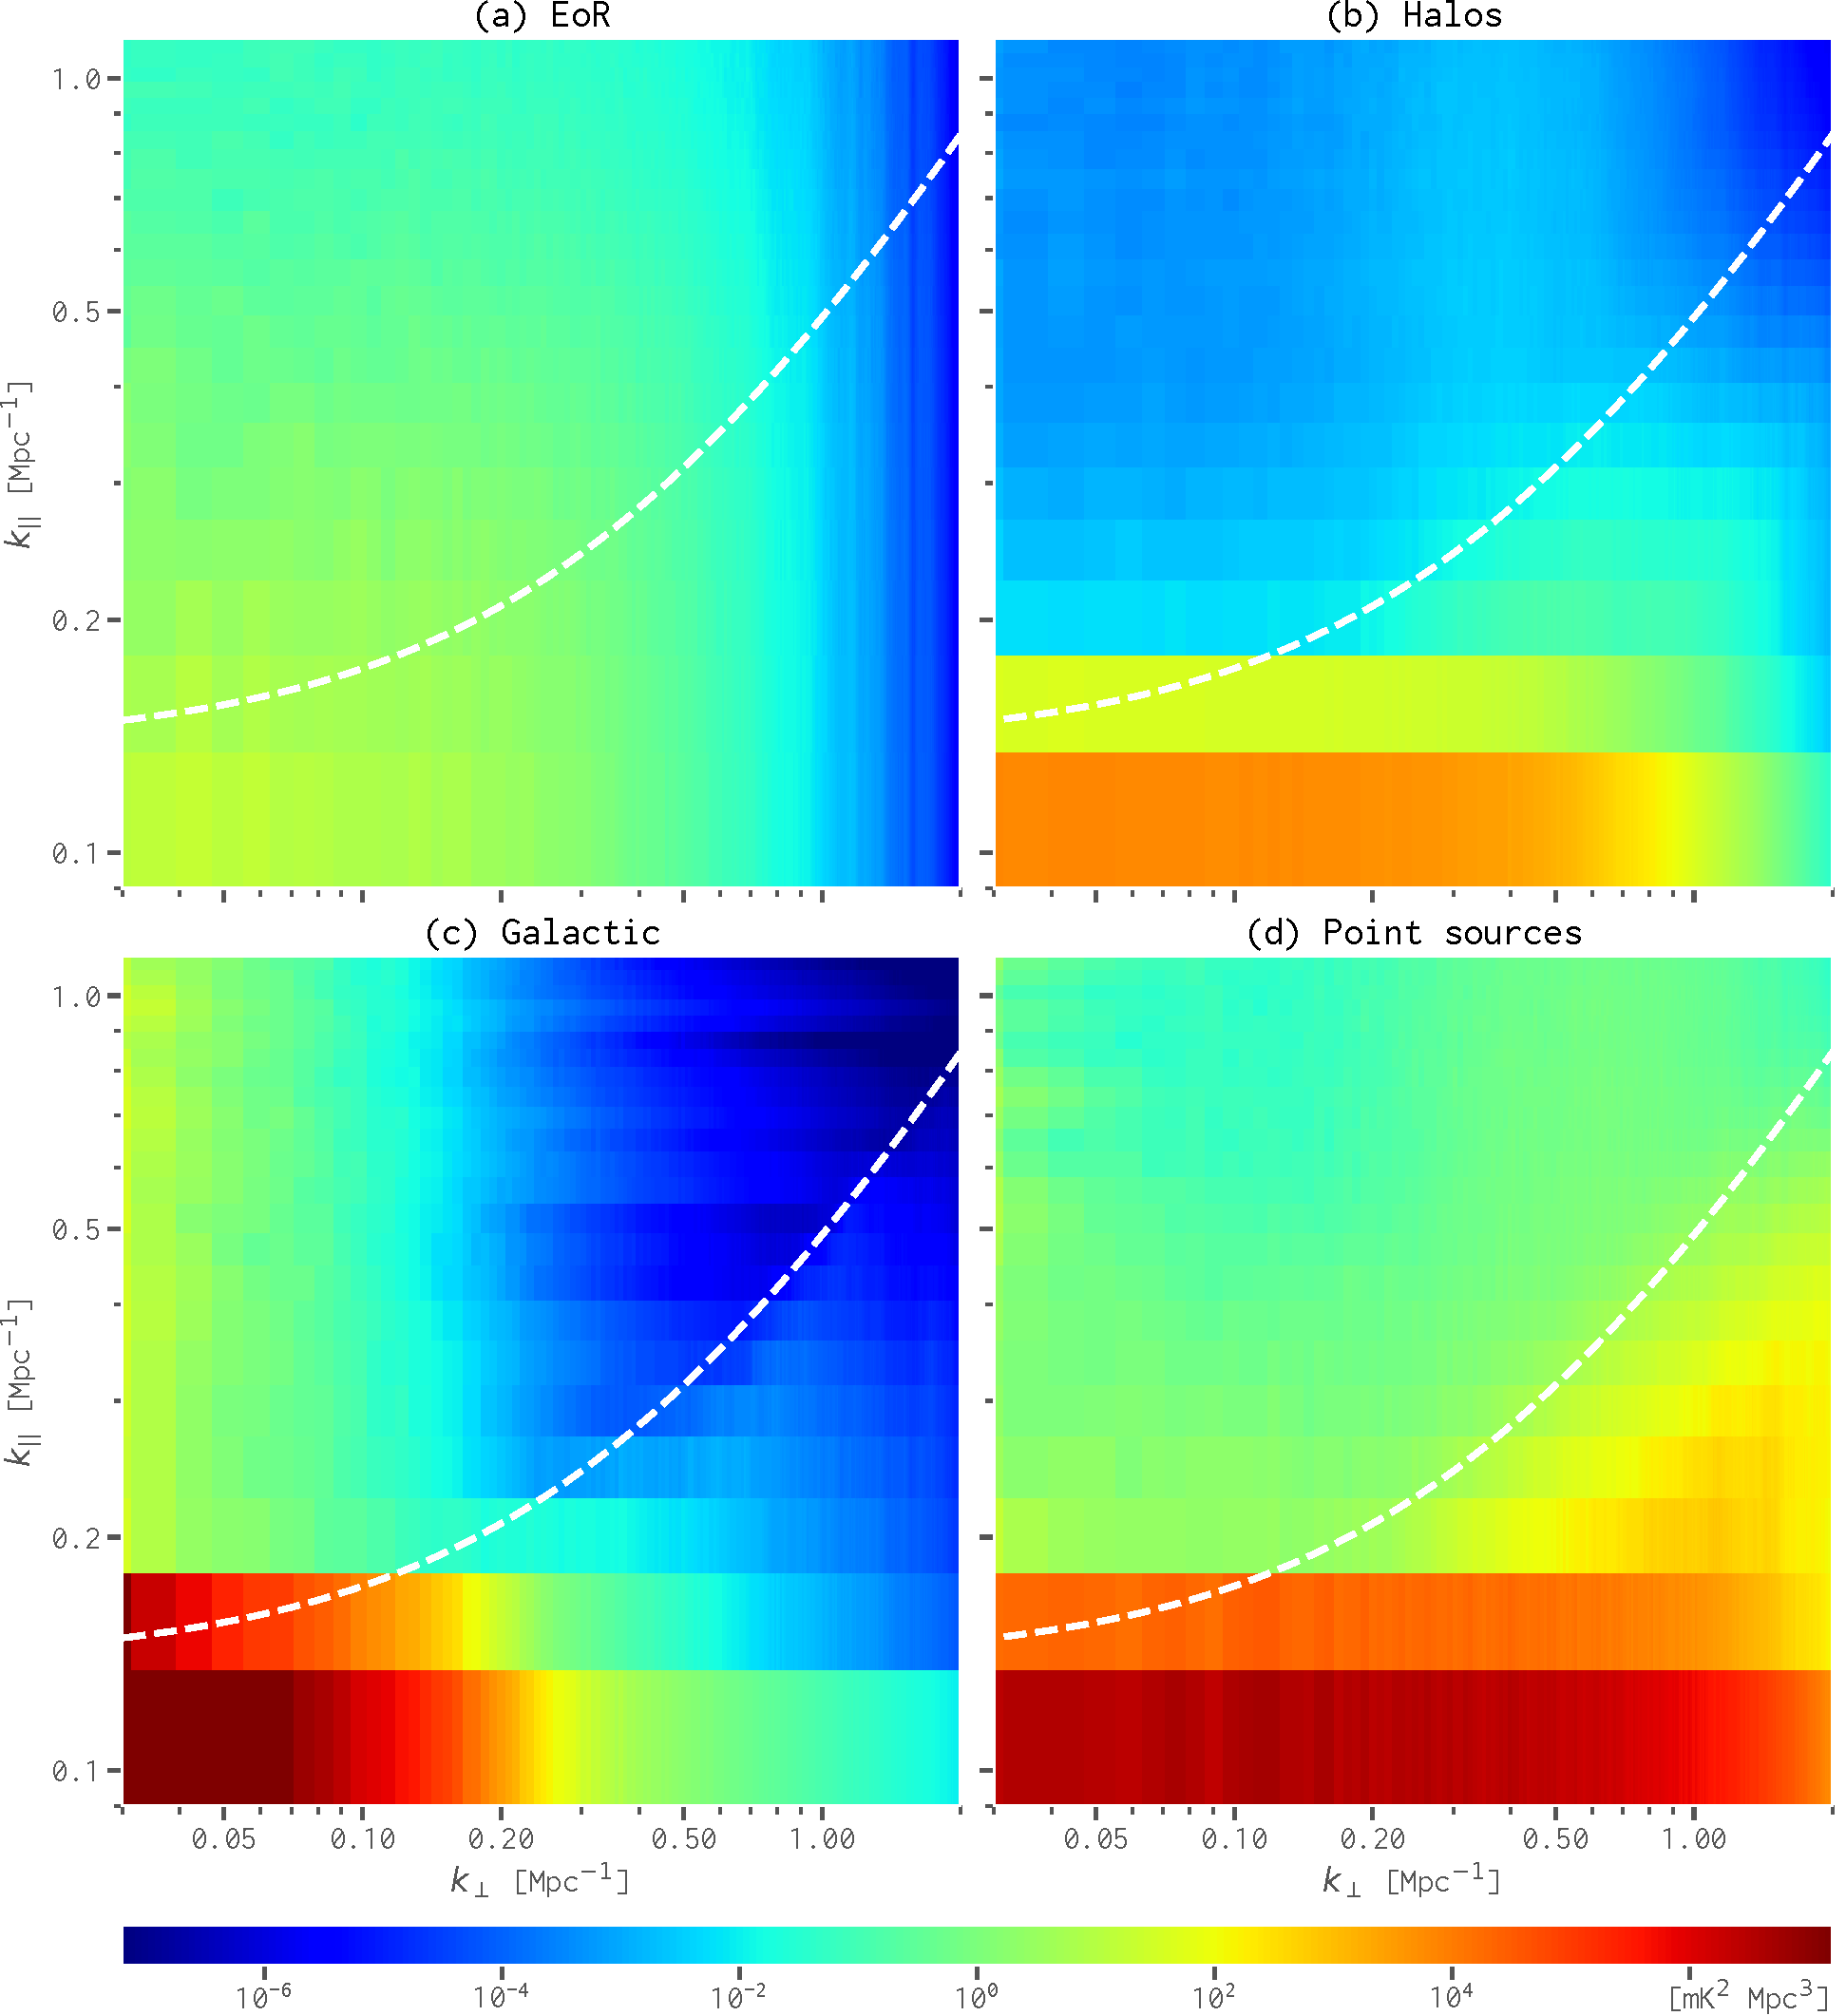
\includegraphics[width=\textwidth]{ps2d-band158}
  \bicaption[EoR 信号和前景成分在 \SIrange{154}{162}{\MHz} 频带的二维功率谱]{%
    各成分在 \SIrange{154}{162}{\MHz} 频带的二维功率谱
    $\ac{psD}(\ac{k-perp}, \ac{k-los})$,
    从左上至右下分别为:
    \emph{(a)} EoR 信号;
    \emph{(b)} 射电晕(100 次模拟的中位值);
    \emph{(c)} 银河系弥散辐射;
    \emph{(d)} 河外点源。
    所有子图共用了以 [\si{\mK\squared\Mpc\cubed}] 为单位的对数\ac{colorbar}。
    白色虚线显示了 EoR 窗口的边界。
  }{%
    The \SIrange{154}{162}{\MHz} 2D power spectra
    $\ac{psD}(\ac{k-perp}, \ac{k-los})$ of
    \emph{(a)} the EoR signal,
    \emph{(b)} radio halos (median of the 100 simulation runs),
    \emph{(c)} Galactic diffuse emission,
    and
    \emph{(d)} extragalactic point sources.
    All panels share the same logarithmic scale in units of
    [\si{\mK\squared\Mpc\cubed}].
    The dashed white lines mark the boundary between the EoR window
    (at the top left) and the contaminating wedge (at the bottom right).
  }
  \label{fig:ps2d}
\end{figure}

以 \SIrange{154}{162}{\MHz} 频带为例,
\autoref{fig:ps2d} 显示了 EoR 信号、射电晕、银河系弥散辐射以及河外点源的
二维功率谱 $\ac{psD}(\ac{k-perp}, \ac{k-los})$,
其中射电晕的二维功率谱对应于 100 次模拟结果的中位值。
从图中容易看出,EoR 信号的功率分散在大范围的 \ac{k-los} \ac{mode}里,
反映了 EoR 信号沿频率维度快速变化的特点;
频谱光滑的前景成分则集中在 \ac{k-los} 较小的区域
($\ac{k-los} \lesssim \SI{0.2}{\per\Mpc}$;
对应于 $\ac{scale} \gtrsim \SI{12}{\arcminute}$)。
在空间维度 (\ac{k-perp}),射电晕辐射的功率主要出现在
$\ac{k-perp} \lesssim \SI{1}{\per\Mpc}$ 的范围,
并且倾向于集中在 $\ac{k-perp} \sim \SI{0.5}{\per\Mpc}$
($\ac{scale} \sim \SI{4.8}{\arcminute}$) 的中等尺度上。
银河系弥散辐射的功率主导了 $\ac{k-perp} \lesssim \SI{0.1}{\per\Mpc}$
($\ac{scale} \gtrsim \SI{24}{\arcminute}$)
的大尺度区域,而河外点源辐射的功率则占据了
$\ac{k-perp} \gtrsim \SI{0.1}{\per\Mpc}$
($\ac{scale} \lesssim \SI{24}{\arcminute}$) 的中小尺度范围。
这些结果与 \autoref{fig:ps1d-3bands}(b) 所示结果相符,
也与诸多文献中的结果一致 \cite{datta2010,trott2015,barry2016,chapman2016}。

\begin{figure}[htp]
  \centering
  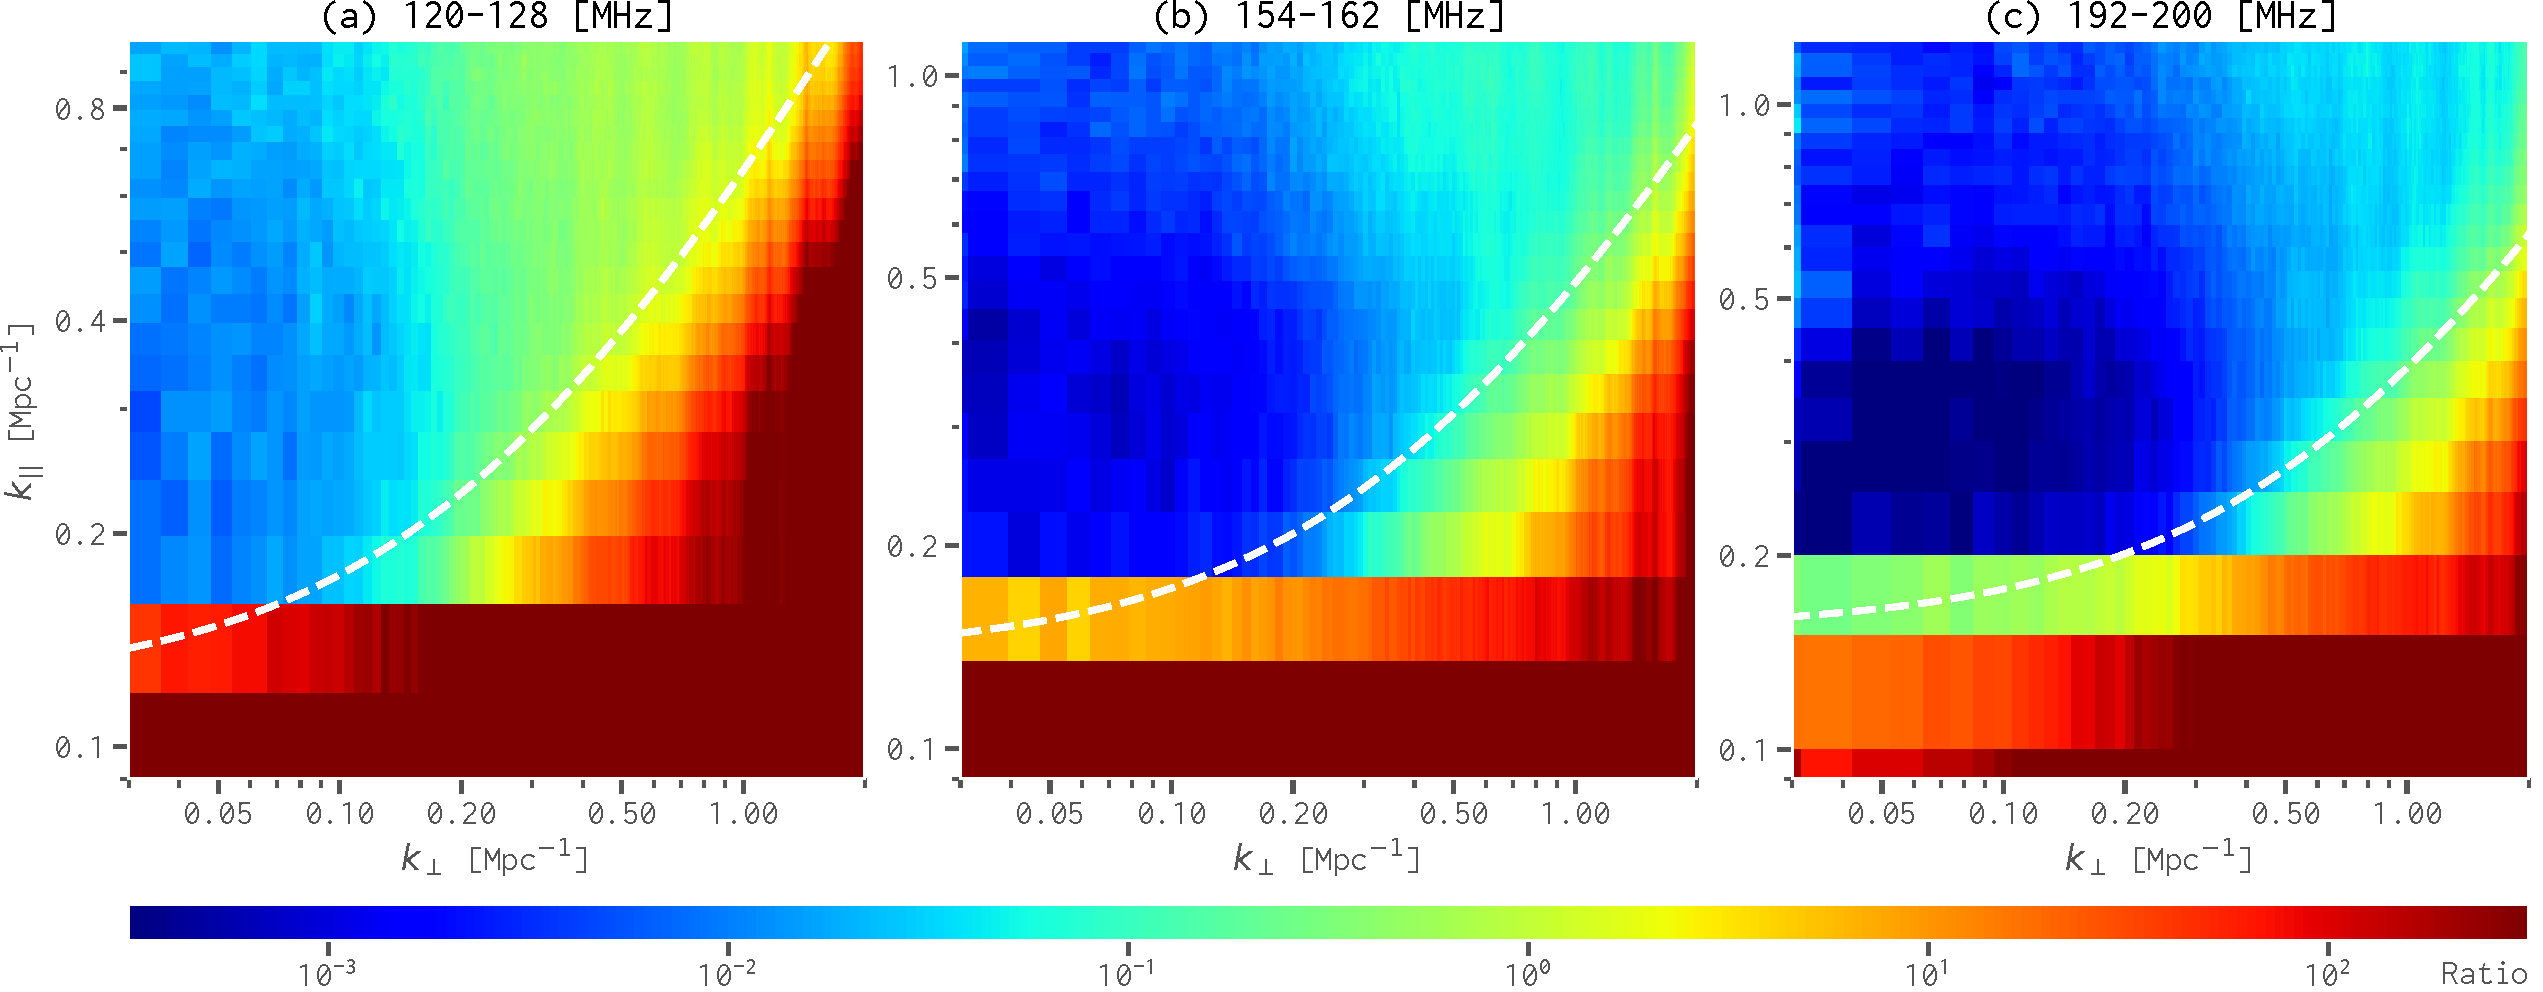
\includegraphics[width=\textwidth]{ps2d-ratio-3bands}
  \bicaption[射电晕和 EoR 信号在三个频带内的二维功率比]{%
    射电晕和 EoR 信号在
    \emph{(a)} \SIrange{120}{128}{\MHz}、
    \emph{(b)} \SIrange{154}{162}{\MHz} 和
    \emph{(c)} \SIrange{192}{200}{\MHz}
    三个频带内的二维功率比 $R(\ac{k-perp}, \ac{k-los})$。
    这里使用的射电晕二维功率谱对应于 100 次模拟结果的中位值。
    所有子图共用了对数\ac{colorbar}。
    白色虚线显示了 EoR 窗口的边界。
  }{%
    The 2D power spectrum ratios $R(\ac{k-perp}, \ac{k-los})$ of
    radio halos to the EoR signal in the
    \emph{(a)} \SIrange{120}{128}{\MHz},
    \emph{(b)} \SIrange{154}{162}{\MHz}, and
    \emph{(c)} \SIrange{192}{200}{\MHz} frequency bands.
    The median 2D power spectrum of 100 simulation runs for radio halos
    is used.
    All panels use the same color bar in logarithmic scale.
    The dashed white lines mark the EoR window boundaries.
  }
  \label{fig:ps2d-ratio}
\end{figure}

为了更具体地显示射电晕辐射对 EoR 信号探测的污染情况,
我们将射电晕辐射的二维功率谱 $\Delta^2_{\R{halo}}(\ac{k-perp}, \ac{k-los})$
除以 EoR 信号的二维功率谱 $\Delta^2_{\R{eor}}(\ac{k-perp}, \ac{k-los})$,
得到两者的二维功率比:
\begin{equation}
  R(\ac{k-perp}, \ac{k-los})
    \equiv \frac{\Delta^2_{\R{halo}}(\ac{k-perp}, \ac{k-los})}{
      \Delta^2_{\R{eor}}(\ac{k-perp}, \ac{k-los})} .
\end{equation}
如\autoref{fig:ps2d-ratio} 所示,
可见射电晕辐射的污染区域形成一个明显的楔形区域 (\autoref{sec:eor-window})。
我们发现,在 \SIrange{120}{128}{\MHz} 频带内,
射电晕辐射在 $\ac{k-perp} \gtrsim \SI{0.1}{\per\Mpc}$
($\ac{scale} \lesssim \SI{22}{\arcminute}$) 的尺度范围内
对 EoR 信号探测产生了严重污染(两者的功率之比达到 $R \gtrsim 1$)。
在 \numrange{154}{162} 和 \numrange{192}{200} \si{\MHz} 两个频带里,
射电晕辐射的主要污染范围分别为 $\ac{k-perp} \gtrsim \SI{0.3}{\per\Mpc}$
($\ac{scale} \lesssim \SI{8}{\arcminute}$)
和 $\ac{k-perp} \gtrsim \SI{0.5}{\per\Mpc}$
($\ac{scale} \lesssim \SI{5}{\arcminute}$)。
注意,尺度 \ac{scale} 与\ac{wavenumber} \ac{k} 之间的换算依赖于频率,
具体可参见附录 \autoref{sec:wavenumber-scale-conv} 的\autoref{tab:k-s-conv}。
另外容易看出,射电晕辐射在较低频率处 ($\sim$\,\SI{120}{\MHz})
对 EoR 探测的污染程度明显强于在较高频率处 ($\sim$\,\SI{200}{\MHz}) 的污染程度。
\autoref{fig:ps1d-3bands} 也显示了与此一致的结果。

\begin{figure}[htp]
  \centering
  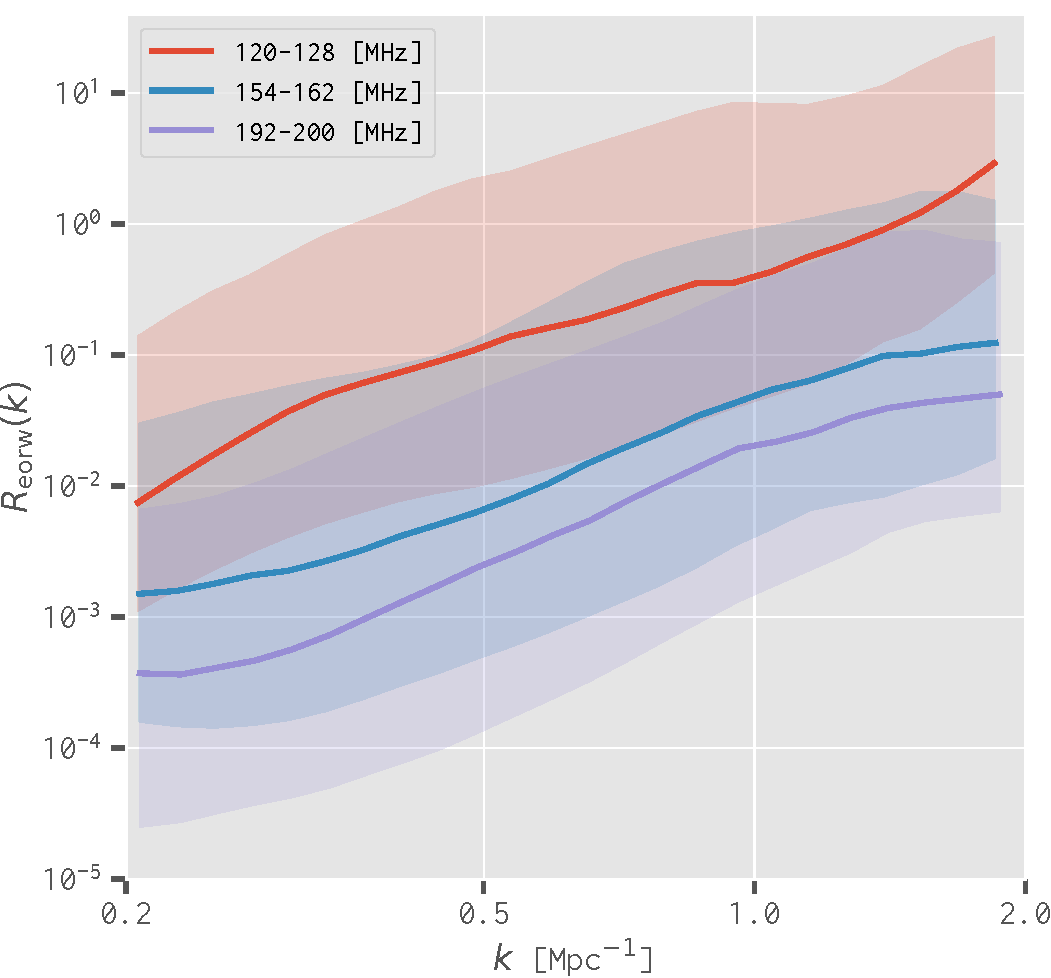
\includegraphics[width=0.8\textwidth]{ps1d-ratio-3bands}
  \bicaption[射电晕和 EoR 信号在 EoR 窗口内的一维功率比]{%
    射电晕和 EoR 信号在 EoR 窗口内的一维功率比 $R_{\R{eorw}}(k)$。
    实线和阴影区域分别对应于射电晕 100 次模拟结果的中位值和 68\% 误差范围。
  }{%
    The 1D power ratios $R_{\R{eorw}}(k)$ inside the EoR window of
    radio halos to the EoR signal.
    The solid lines and shaded regions show the median values and
    corresponding 68\% uncertainties, respectively.
  }
  \label{fig:ps1d-ratio}
\end{figure}

考虑到射电晕辐射的污染主要集中在二维功率谱右下方的楔形区域内
(如\autoref{fig:ps2d-ratio} 所示),
因此可以选定一个合适的边界将其排除,
于是能够在左上方的 EoR 窗口内提取 EoR 信号,
有效地避开了强烈的前景污染,这就是\ac{fg-avd}方法的基本思路
(参见 \autoref{sec:eor-window})。
根据\autoref{eq:eor-window} 定义的 EoR 窗口边界的表达式,
我们测试了多种不同的 $(\psi,\, \Phi)$ 参数组合,
最终选择了 $\psi = 3$ 以及 $\Phi = 1.5\,\ac{Fov}$,
其中 \ac{Fov} 为\acl{Fov};
所以 $\Phi$ 在 \numrange{120}{128}、\numrange{154}{162}
和 \numrange{192}{200} \si{\MHz} 三个频带的值分别为
$\Phi_{124} = \SI{7.5}{\degree}$、
$\Phi_{158} = \SI{6.0}{\degree}$ 和
$\Phi_{196} = \SI{4.8}{\degree}$。
\autoref{fig:ps2d} 和\autoref{fig:ps2d-ratio} 显示了如此定义的 EoR 窗口边界,
可见\ac{fg-wedge}的污染能够被很好地避开。
但是在 \numrange{120}{128}、\numrange{154}{162}
和 \numrange{192}{200} \si{\MHz} 三个频带内,
EoR 信号分别有约 45\%、46\% 和 60\% 的功率损失在避开的\ac{fg-wedge}之中。

在上述定义的 EoR 窗口内,对射电晕辐射与 EoR 信号的二维功率比
$R(\ac{k-perp}, \ac{k-los})$ 进行平均,
可得到一维功率比 $R_{\R{eorw}}(k)$,如\autoref{fig:ps1d-ratio} 所示。
相比\autoref{fig:ps1d-3bands} 所示的未受 EoR 窗口约束的一维功率谱 $\ac{psD}(k)$,
射电晕辐射的污染在 EoR 窗口内被抑制了约 4 个数量级。
比如,在 $k \sim \SI{1}{\per\Mpc}$
(约对应于 $\ac{scale} \sim \SI{2.4}{\arcminute}$)尺度上,
EoR 窗口内的一维功率比 $R_{\R{eorw}}(k)$ 在 \numrange{120}{128}、
\numrange{154}{162} 和 \numrange{192}{200} \si{\MHz}
三个频带的典型值(图中的实线)分别约为 45\%、6\% 和 2\%。
这充分展示了 EoR 窗口和\ac{fg-avd}法是探测 EoR 信号的有力工具。
尽管如此,由于射电晕的亮度和数目在不同天区里具有显著的涨落,
在 68\% 误差范围(图中的阴影区域)以及
$\SI{0.5}{\per\Mpc} \lesssim k \lesssim \SI{1}{\per\Mpc}$
(约对应于 $\SI{2.4}{\arcminute} < \ac{scale} < \SI{4.8}{\arcminute}$)
尺度范围内,
EoR 窗口内的一维功率比 $R_{\R{eorw}}(k)$ 在三个频带内的值能够分别达到约
\numrange{230}{800}\%、\numrange{18}{95}\% 和 \numrange{7}{40}\%,
说明射电晕泄漏到 EoR 窗口内的功率仍然可能是显著的,
尤其是在较低频率 ($\lesssim$\,\SI{120}{\MHz})。

基于本节和上一节 (\autoref{sec:ps1d}) 的结果,
我们认为射电晕是 EoR 信号探测的一个重要前景干扰成分。
即使在已避开严重污染的 EoR 窗口内,
射电晕辐射所产生的污染仍然能够对 EoR 信号的准确测量产生不可忽略的干扰,
尤其是在 $\lesssim$\,\SI{120}{\MHz} 的较低频率。
为了获得一个尽可能干净、同时也尽可能大的 EoR 窗口,
必须深入理解、建模并扣除射电晕以及其他前景干扰成分。
同时还需要联合使用\ac{fg-rm}和\ac{fg-avd}两类方法,
改进 EoR 信号探测手段 \cite{kerrigan2018}。


%=====================================================================
\section{频谱伪结构的影响}
\label{sec:freq-artifacts}

射电干涉观测的实际情况比 \autoref{sec:obs-simu} 所模拟的理想情况要复杂得多,
比如面临不理想的仪器校准,电离层的扰动(参见 \autoref{sec:det-difficulties})。
这些复杂的仪器效应和观测效应会导致\ac{imgcube}的频谱出现伪结构,
破坏前景辐射的频谱光谱性,从而阻碍 EoR 信号的有效分离。

一些模拟和观测研究指出,干涉阵列频率\ac{channel}的校准存在约
\numrange{0.1}{1}\% 的不确定性
\cite{barry2016,beardsley2016,ewallWice2017}。
为了评估这种频谱伪结构对\ac{ps}以及前景干扰的影响,
我们对\ac{imgcube}的每一个\ac{slice}乘以
一个从平均值为 0、标准差为 σ 的正态分布生成的随机数,
以此模拟实际观测中出现的频谱伪结构 \cite{chapman2016},
然后计算有无频谱伪结构的\ac{imgcube}的\ac{ps}并进行对比。
本文考虑如下两种边界情况:
\begin{itemize}
  \item 频谱伪结构的幅度为 $A_{\R{arti}} = 0.1\%$,
    对应于正态分布的标准差为 $σ = 0.001$;
  \item 频谱伪结构的幅度为 $A_{\R{arti}} = 1\%$,对应于 $σ = 0.01$。
\end{itemize}

\begin{figure}[htp]
  \centering
  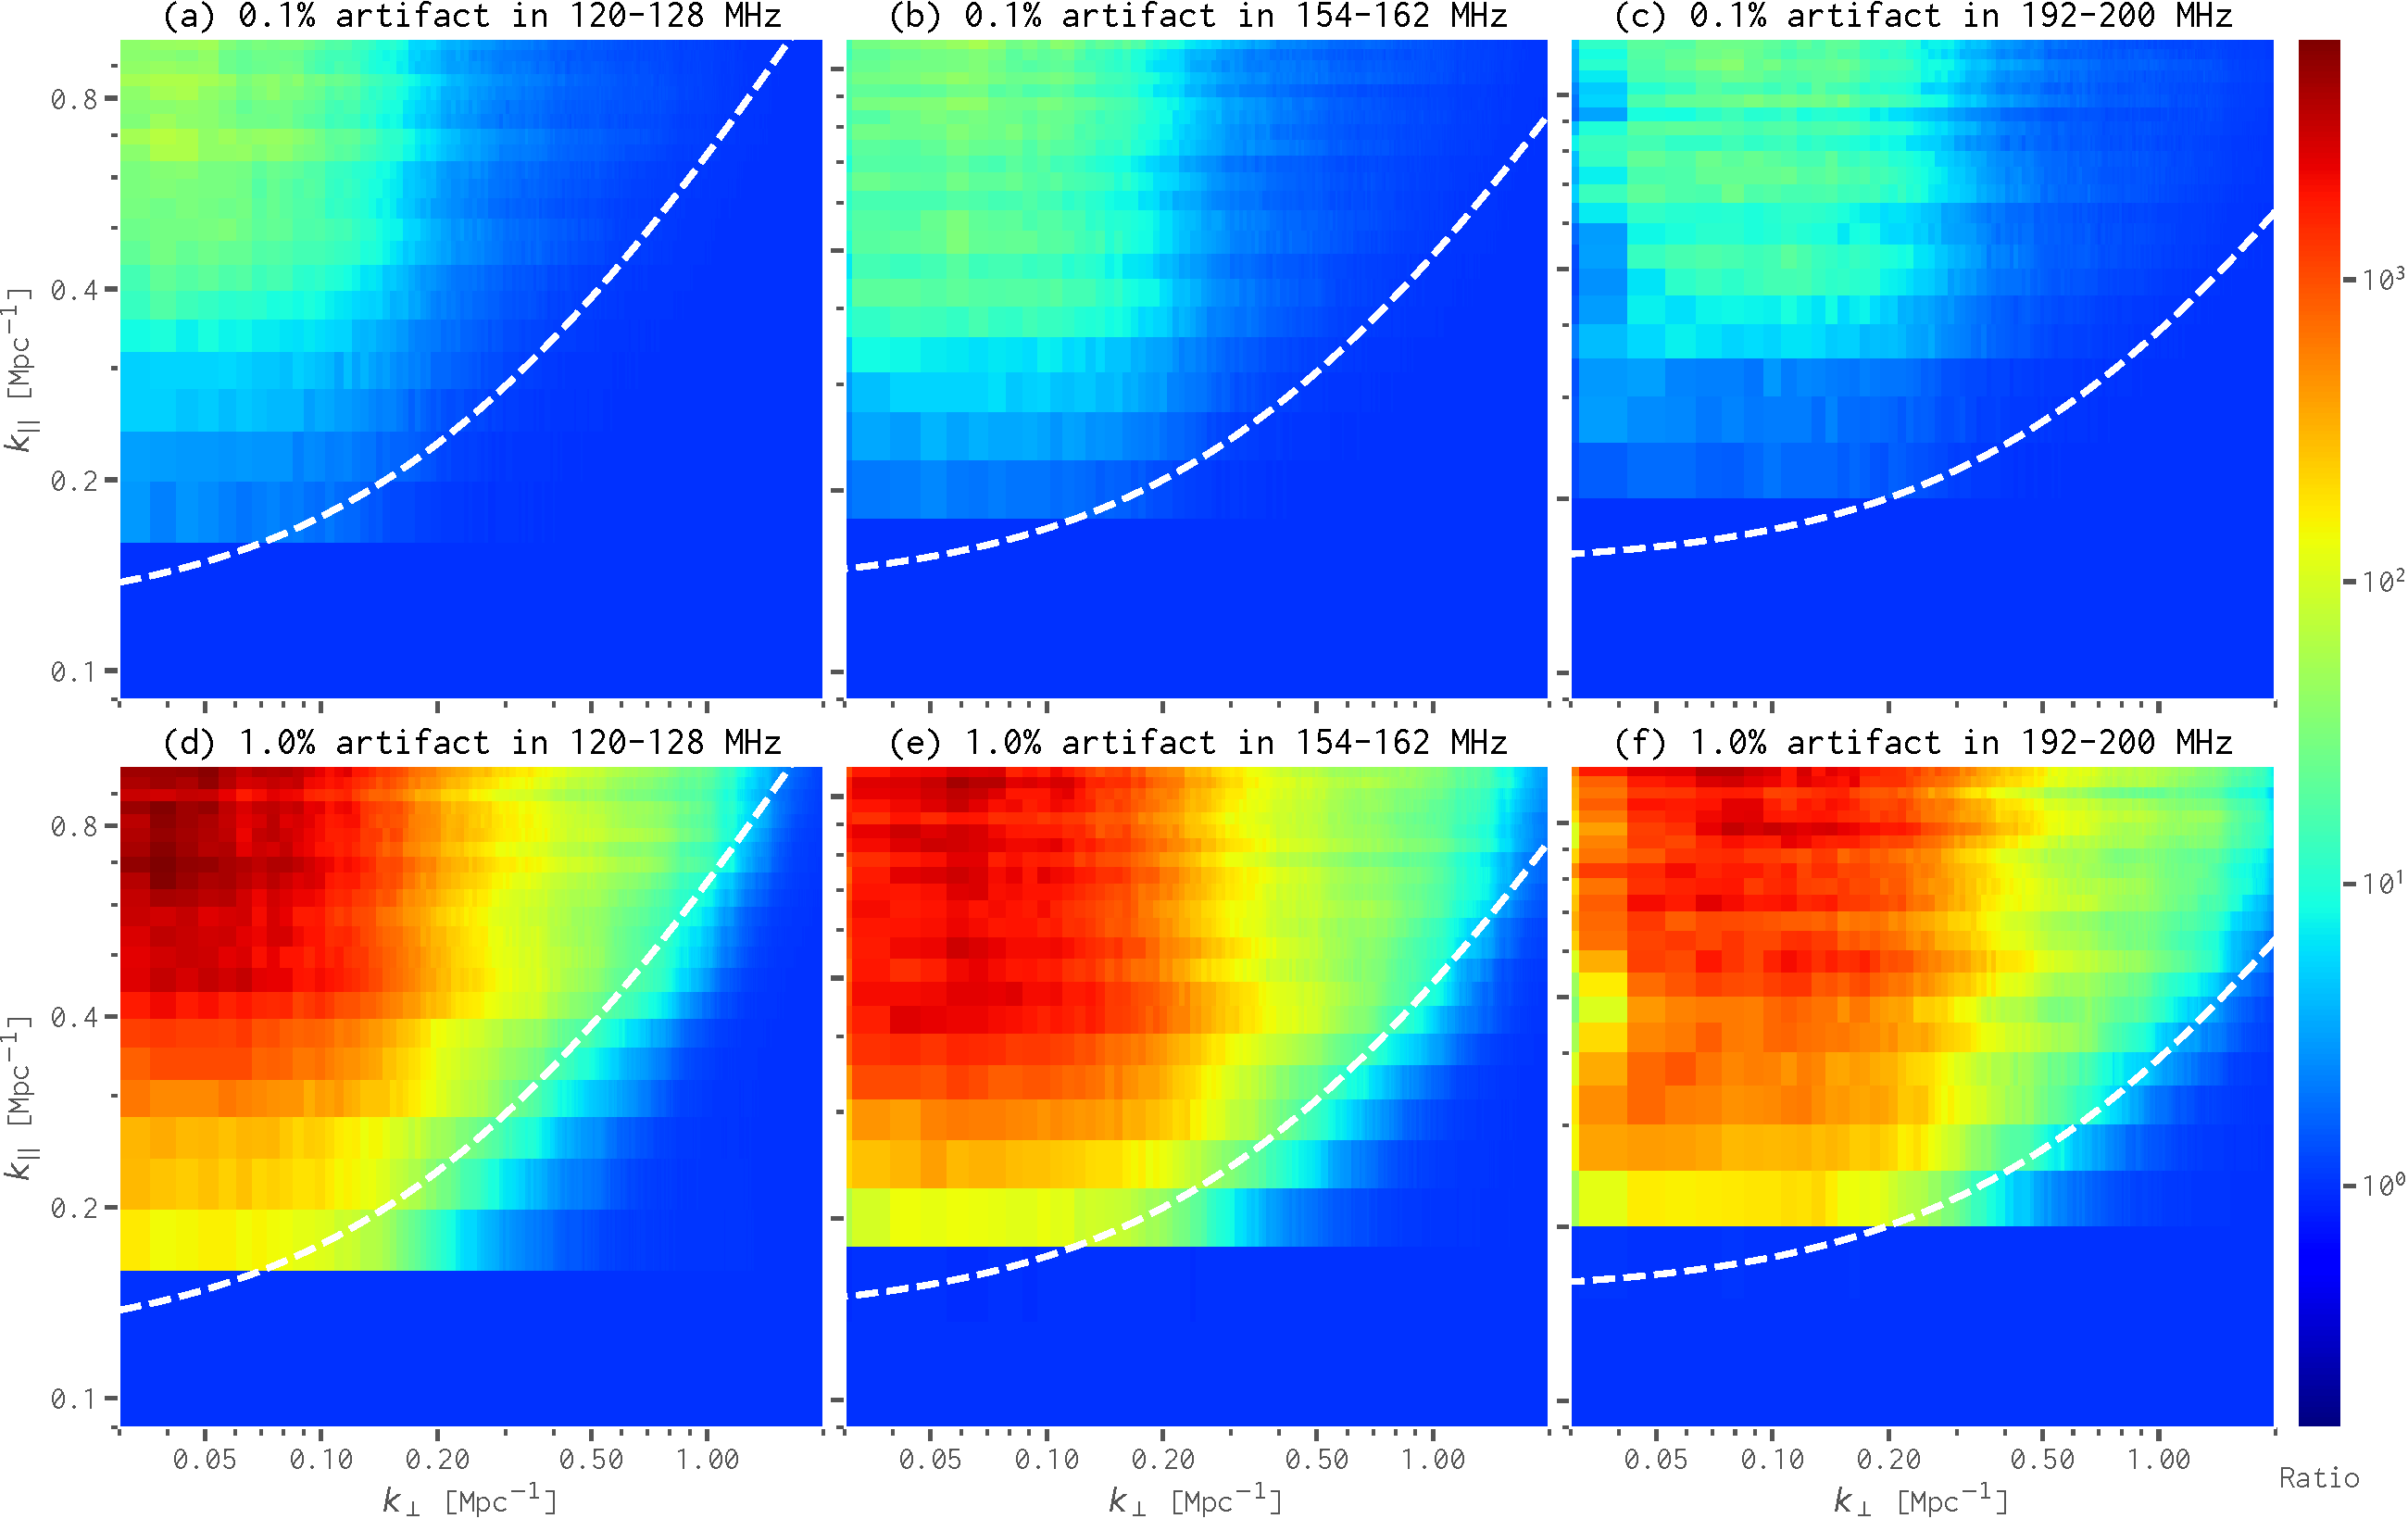
\includegraphics[width=0.75\textwidth]{ps2d-ratio-crp-3bands}
  \bicaption[有无频谱伪结构时射电晕的二维功率比]{%
    有无频谱伪结构时射电晕的二维功率比 $R_{\R{arti}}(\ac{k-perp}, \ac{k-los})$。
    上、中、下三行分别对应 \numrange{120}{128}、\numrange{154}{162} 和
    \numrange{192}{200} \si{\MHz} 三个频带;
    左、右两列分别显示了频谱伪结构幅度为 $A_{\R{arti}} = 0.1\%$
    和 $A_{\R{arti}} = 1\%$ 的情况;
    白色虚线标识了 EoR 窗口的边界。
    所有子图共用了对数\ac{colorbar}。
  }{%
    The 2D power spectrum ratios $R_{\R{arti}}(\ac{k-perp}, \ac{k-los})$
    of radio halos with and without frequency artifacts.
    The upper, middle, and lower rows show the power spectrum ratios
    in the \numrange{120}{128}, \numrange{154}{162}, and
    \numrange{192}{200} \si{\MHz} bands, respectively;
    the left and right columns show the cases of frequency artifacts
    being $A_{\R{arti}} = 0.1\%$ and $A_{\R{arti}} = 1\%$, respectively.
    The dashed white lines mark the EoR window boundaries.
    All panels share the same color bar in logarithmic scale.
  }
  \label{fig:ps2d-ratio-crp}
\end{figure}

给定一个\ac{imgcube},计算在有频谱伪结构和无频谱伪结构情形下的二维功率谱,
分别为 $\Delta^2_{\R{arti}}(\ac{k-perp}, \ac{k-los})$
和 $\Delta^2(\ac{k-perp}, \ac{k-los})$,
于是可得两者之比为:
\begin{equation}
  R_{\R{arti}}(\ac{k-perp}, \ac{k-los})
    \equiv \frac{\Delta^2_{\R{arti}}(\ac{k-perp}, \ac{k-los})}{
      \Delta^2(\ac{k-perp}, \ac{k-los})} .
\end{equation}
对于射电晕的 100 次模拟,我们计算了每一次模拟在 \numrange{120}{128}、
\numrange{154}{162} 和 \numrange{192}{200} \si{\MHz} 三个频带内、
频谱伪结构幅度为 $A_{\R{arti}} = 0.1\%$ 和 $A_{\R{arti}} = 1\%$
情形下的二维功率比 $R_{\R{arti}}(\ac{k-perp}, \ac{k-los})$,
得到了射电晕辐射在三个频带内以及两种频谱伪结构幅度的情况下的二维功率比的中位值,
结果如\autoref{fig:ps2d-ratio-crp} 所示。
我们发现,射电晕辐射的二维功率谱受到了频谱伪结构的严重破坏。
在 $\ac{k-perp} \lesssim \SI{0.2}{\per\Mpc}$ 和
$\ac{k-los} \gtrsim \SI{0.3}{\per\Mpc}$ 尺度范围内,
幅度为 $A_{\R{arti}} = 0.1\%$ 的频谱伪结构使射电晕在 \numrange{120}{128}、
\numrange{154}{162} 和 \numrange{192}{200} \si{\MHz}
三个频带内的功率分别增加了约 17、15 和 13 倍。
当频谱伪结构的幅度为 $A_{\R{arti}} = 1\%$,即为前一种情况的 10 倍时,
射电晕辐射在相同尺度范围内的功率比 $R_{\R{arti}}$ 则为前一种情况的 100 倍,
即在三个频带内分别约为 1700、1500 和 1300。

作为对比,我们对 EoR 信号的\ac{imgcube}引入了同样的频谱伪结构
($A_{\R{arti}} = 0.1\%$ 或 $1\%$)
并计算了相应的二维功率比 $R_{\R{arti}}(\ac{k-perp}, \ac{k-los})$,
但是发现 EoR 信号的二维功率谱几乎未受频谱伪结构的影响,
即使频谱伪结构的幅度为 $A_{\R{arti}} = 1\%$。
这主要是因为 EoR 信号在频率维度已经具有明显的小尺度起伏结构。

由上述结果可知,即便是非常微小(幅度约为 $\sim$\,0.1\%)的频谱伪结构
也会使射电晕辐射的干扰显著增强,特别是在关键的 EoR 窗口内。
这说明 EoR 探测实验需要对仪器进行非常严格的校准,
以获得非常准确的频谱响应 \cite{barry2016}。
这些结果也进一步支持射电晕对 EoR 探测而言是一个严重的前景干扰成分。


%=====================================================================
\section{旁瓣内射电晕辐射的影响}
\label{sec:fscn}

\begin{figure}[htp]
  \centering
  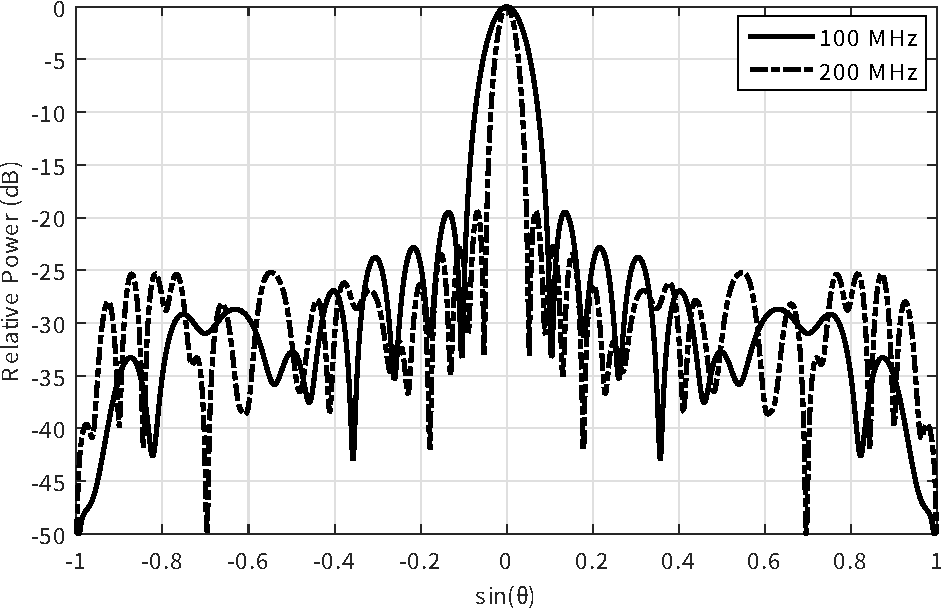
\includegraphics[width=0.8\textwidth]{SKA1-low-beams}
  \bicaption{%
    SKA1-Low 在 100 和 200 MHz 处的模拟站点波束
  }{%
    The simulated station beams of SKA1-Low at 100 and 200 MHz.
    \\来源/Credit:
    \citeay{mort2017} [删减了标识]
  }
  \label{fig:ska-beams}
\end{figure}

低频干涉阵列的波束形状非常复杂,除\ac{mainlobe}外还有一系列明显的\ac{sidelobe}
\cite{noordam2004,wijnholds2010}(\autoref{fig:ska-beams}),
更多关于 SKA1-Low 的波束形状及其影响的研究可参见 \citeay{mort2017}。
辐射源即使远在视场之外,也会通过\ac{sidelobe}在视场中产生类似噪声的干扰,
即\acf{fscn} \cite{smirnov2012}。
更加重要的是,当观测的 $uv$ 覆盖达到饱和时,\ac{fscn} 便不再降低,
因此 \ac{fscn} 可能会超过仪器热噪声而成为制约成像质量的关键因素之一 \cite{mort2017}。

为了研究\ac{sidelobe}内的射电晕所产生的 \ac{fscn},
我们需要生成相应的天图并模拟包含仪器效应的 SKA1-Low 观测图像。
\texttt{OSKAR} 利用了射电干涉仪测量方程 (measurement equation) \cite{smirnov2011},
实现了高仿真的\ac{beam-forming},并且能够开展全天模拟 \cite{mort2010}。
我们取 \SIrange{154}{162}{\MHz} 频带为例,
首先模拟射电晕的天图,其中射电晕覆盖了从第二\ac{sidelobe}的边缘
(距离视场中心 $\phi \sim \SI{10}{\degree}$)
一直到地平线 ($\phi = \SI{90}{\degree}$) 的范围。
这相当于在实际数据处理中将\ac{mainlobe}和第一\ac{sidelobe}里的射电晕
全部识别并完全去除。
然后,使用 \texttt{OSKAR} 和 \texttt{WSClean} 软件按
\autoref{sec:obs-simu} 所述方法进行模拟观测并成像,
得到视场中央 \SI{5 x 5}{\degree} 区域的\ac{map-dirty}。
因为视场(即\ac{mainlobe})内没有辐射源,没有必要、也无法进行 CLEAN,
所以直接从\ac{vis}数据生成\ac{map-dirty}即可。
对频带内的所有频率\ac{channel}均如此处理,
于是得到射电晕 \ac{fscn} 的\ac{imgcube},
最后计算其二维功率谱 $\Delta^2_{\R{fscn}}(\ac{k-perp}, \ac{k-los})$。

\begin{figure}[htp]
  \centering
  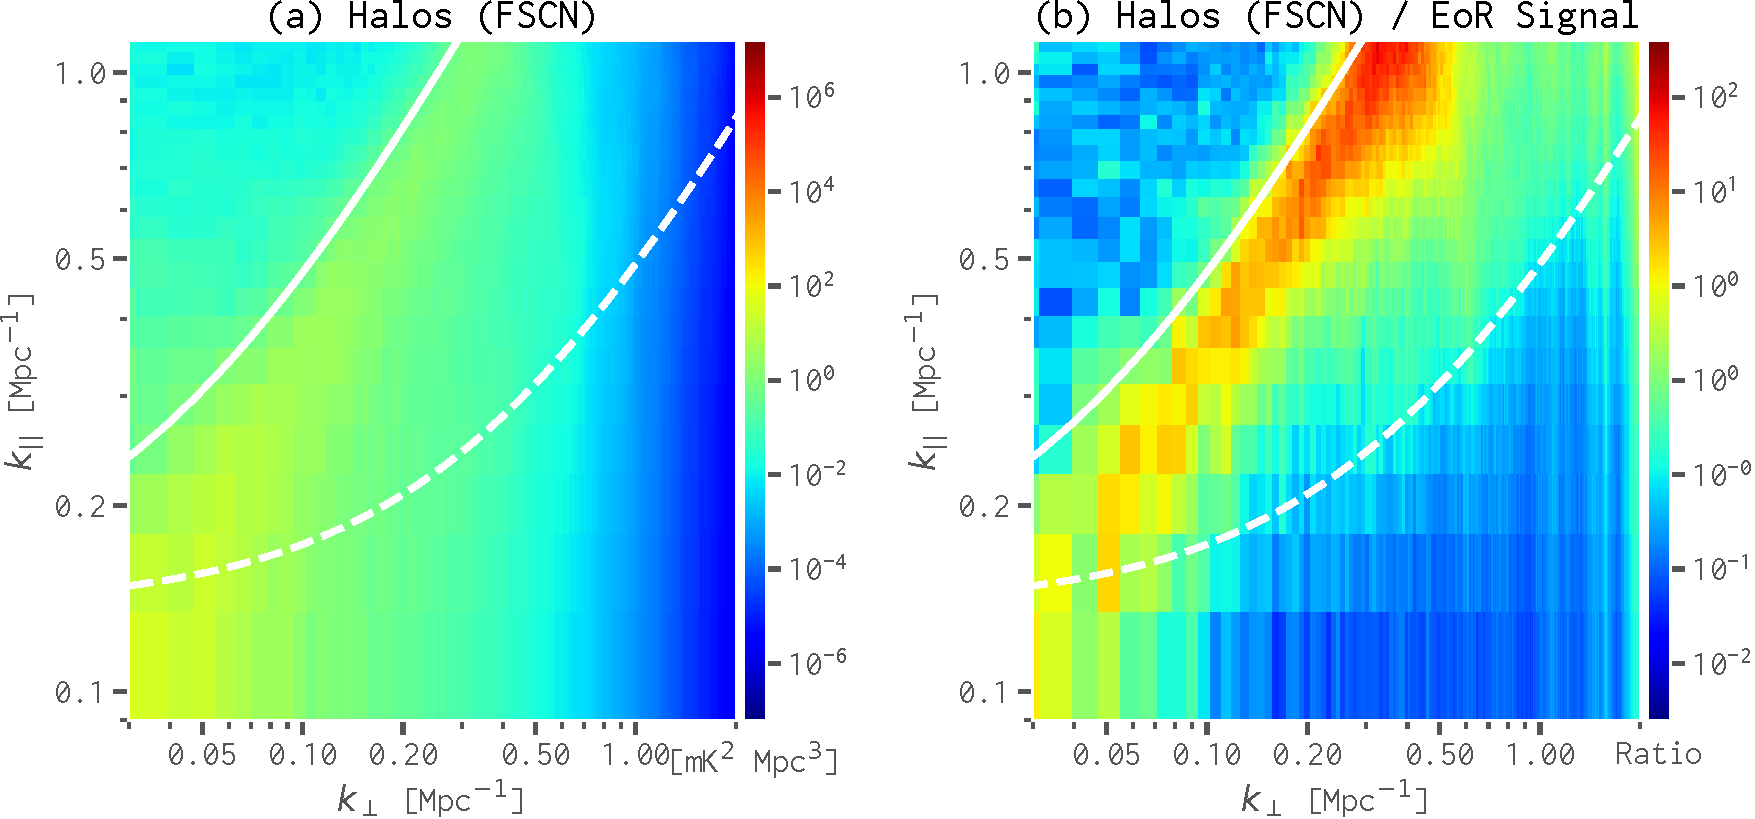
\includegraphics[width=\textwidth]{ps2d-fscn}
  \bicaption[射电晕 FSCN 的二维功率谱及其与 EoR 信号的功率谱对比]{%
    (\uline{左栏}) 射电晕 FSCN 的二维功率谱
      $\Delta^2_{\R{fscn}}(\ac{k-perp}, \ac{k-los})$;
    (\uline{右栏}) 射电晕 FSCN 与 EoR 信号的二维功率比
      $R_{\R{fscn}}(\ac{k-perp}, \ac{k-los})$。
    白色虚线和实线分别标识了 $\Phi = \SI{6.0}{\degree}$ 和 \SI{90}{\degree}
    所对应的 EoR 窗口边界。
  }{%
    (\uline{Left}) The 2D power spectrum of the FSCN caused by radio halos
    in the far side-lobes of the station beam.
    (\uline{Right}) The 2D power spectrum ratio of the FSCN to the EoR signal.
    The results are derived in the \SIrange{154}{162}{\MHz} band.
    The dashed and solid white lines mark the EoR window boundaries
    defined with $\Phi = \SI{6.0}{\degree}$ and \SI{90}{\degree},
    respectively.
  }
  \label{fig:ps2d-fscn}
\end{figure}

\autoref{fig:ps2d-fscn} 显示了射电晕 \ac{fscn}
的二维功率谱 $\Delta^2_{\R{fscn}}(\ac{k-perp}, \ac{k-los})$
以及与 EoR 信号的二维功率比 $R_{\R{fscn}}(\ac{k-perp}, \ac{k-los})$。
我们发现,射电晕 \ac{fscn} 对 EoR 信号产生的干扰非常严重:
在 $\ac{k-perp} \sim \SI{0.3}{\per\Mpc}$
和 $\ac{k-los} \sim \SI{1.0}{\per\Mpc}$ 的附近尺度上,
射电晕 \ac{fscn} 的功率达到了 EoR 信号的约 20 倍。
显然可见,\ac{fg-wedge}污染区域越过了原来的边界(白色虚线)向左上方大幅扩张,
极大地压缩了 EoR 窗口的大小。
为了能够在二维功率谱上有效地避开 \ac{fscn} 的污染,
我们被迫采用一个更加保守的 EoR 窗口边界,
如图中白色实线所示、由 $\Phi = \SI{90}{\degree}$ 确定的边界,
但是如此将损失绝大部分 ($\sim$\,96\%) 的 EoR 信号。

因此,严重的 \ac{fscn} 污染使得筛选 EoR 观测天区成为一个更加困难的任务,
这是因为在原则上不仅在\ac{mainlobe}里,还有在\ac{sidelobe}里,
都不允许出现明亮的射电晕以及其他干扰源。
否则需要在一个远远大于视场的天区里准确识别、建模并扣除这些干扰源,
如此将使数据处理的难度大大提高 \cite{pober2013,pober2016}。


%=====================================================================
\section{小结}

利用\autoref{chap:simulation}模拟的 SKA1-Low 观测图像,
我们对比了射电晕、EoR 信号以及其他前景成分的一维和二维\ac{ps},
充分说明了射电晕是一个重要的前景干扰成分。
即便采用\ac{fg-avd}方法在二维\ac{ps}上避开强烈的前景污染区域,
射电晕辐射在 EoR 窗口内所产生的污染仍然能对 EoR 信号的测量产生不可忽略的影响,
尤其是在 $\lesssim$\,\SI{120}{\MHz} 较低频率。
此外,我们还考虑了仪器的频谱伪结构对射电晕的功率谱的影响,
以及\ac{sidelobe}内的射电晕辐射对 EoR 信号探测的影响。
这些结果进一步说明了射电晕作为前景成分的重要性。

本章内容已发表于 \textit{The Astrophysical Journal} \cite{li.halo}。


%% EOF
